\documentclass[12pt]{article}
\usepackage{siunitx} % Fornece suporte para a tipografia de unidades do Sistema Internacional e formatação de números
\usepackage{booktabs} % Melhora a qualidade das tabelas
\usepackage{tabularx} % Permite tabelas com larguras de colunas ajustáveis
\usepackage{graphicx} % Suporte para inclusão de imagens
\usepackage{newtxtext} % Substitui a fonte padrão pela Times Roman
\usepackage{ragged2e} % Justificação de texto melhorada
\usepackage{setspace} % Controle do espaçamento entre linhas
\usepackage[a4paper, left=3.0cm, top=3.0cm, bottom=2.0cm, rigH=2.0cm]{geometry} % Personalização das margens do documento
\usepackage{lipsum} % Geração de texto dummy 'Lorem Ipsum'
\usepackage{fancyhdr} % Customização de cabeçalhos e rodapés
\usepackage{titlesec} % Personalização dos títulos de seções
\usepackage[portuguese]{babel} % Adaptação para o português (nomes e hifenização)
\usepackage{hyperref} % Suporte a hiperlinks
\usepackage{indentfirst} % Indentação do primeiro parágrafo das seções
\usepackage{siunitx} % (Este pacote está duplicado, você pode querer removê-lo)
\sisetup{
  output-decimal-marker = {,},
  inter-unit-product = \ensuremath{{}\cdot{}},
  per-mode = symbol
}
\DeclareSIUnit{\real}{R\$}
\newcommand{\real}[1]{R\$#1}
\usepackage{float} % Melhor controle sobre o posicionamento de figuras e tabelas
\usepackage{footnotehyper} % Notas de rodapé clicáveis em combinação com hyperref
\usepackage{hyperref} % (Este pacote está duplicado, você pode querer ajustar isso)
\hypersetup{
    colorlinks=true,
    linkcolor=black,
    filecolor=magenta,      
    urlcolor=cyan,
    pdfborder={0 0 0},
}
\usepackage[normalem]{ulem} % Permite o uso de diferentes tipos de sublinhados sem alterar o \emph{}
\makeatletter
\def\@pdfborder{0 0 0} % Remove a borda dos links
\def\@pdfborderstyle{/S/U/W 1} % Estilo da borda dos links
\makeatother
\onehalfspacing

\begin{document}

\begin{titlepage}
    \centering
    \vspace*{1cm}
    \Large\textbf{INSPER – INSTITUTO DE ENSINO E PESQUISA}\\
    \Large \textbf{ECONOMIA}\\
    \vspace{1.5cm}
    \Large\textbf{Atividade Prática Superviosionada II}\\
    \textbf{Econometria}\\
    \vspace{1.5cm}
    Profa. Adriana Bruscato Bortoluzzo\\
    Profa. Auxiliar Renata Serson \\
    \vfill
    \normalsize
    Arthur Salles Mattos Nogueira, \href{mailto:arthursmn@al.insper.edu.br}
    {arthursmn@al.insper.edu.br}\\
    Diogo Roecker Cardozo, \href{mailto:diogorc@al.insper.edu.br}
    {diogorc@al.insper.edu.br}\\
    Fabrizio Antonini Ripoli, \href{mailto:fabrizioar@al.insper.edu.br}{fabrizioar@al.insper.edu.br}\\
    Hicham Munir Tayfour, \href{mailto:hichamt@al.insper.edu.br}{hichamt@al.insper.edu.br}\\
    Matheus Tahan Cunha, \href{mailto:matheustc2@al.insper.edu.br}
    {matheustc2@al.insper.edu.br}\\
    Victor Delgado Dias, \href{mailto:victord1@al.insper.edu.br}
    {victord1@al.insper.edu.br}\\
    4º Período - Economia B\\
    \vfill
    São Paulo\\
    Março/2024
\end{titlepage}

\newpage
\tableofcontents
\thispagestyle{empty} % This command removes the page number from the table of contents page
\newpage
\setcounter{page}{1} % This command sets the page number to start from this page
\justify
\onehalfspacing

\pagestyle{fancy}
\fancyhf{}
\rhead{\thepage}

\section{\textbf{ATENÇÃO SOBRE ESTE ARQUIVO}}
Nas Partes 2 da APS, cada equipe deverá entregar um relatório (MÁXIMO 
20 PÁGINAS). Essas 20 páginas incluem capa, porém não estão incluídos eventuais 
anexos.

\section{\textbf{Base Geral}}
\begin{table}[H]
\centering
\caption{Tabela Descritiva Geral}
\label{tab:indicadores_gerais}
\small
\begin{tabularx}{\textwidth}{l*{6}{R}}
\hline
Indicador & Média & Mediana & Máximo & Mínimo & Variância & Desvio Padrão \\ \hline
Homicídio por 100.000 & 7.59 & 6.65 & 23.70 & 0.00 & 24.91 & 4.99 \\
Armas por 100.000 & 3026.17 & 2344.33 & 24547.23 & 445.49 & 11607970.35 & 3407.05 \\
PIB Per Capita & 61870.72 & 60464.50 & 83461.00 & 49071.00 & 68025916.33 & 8247.78 \\
Taxa de Urbanização & 0.72 & 0.73 & 0.94 & 0.35 & 0.02 & 0.15 \\
Polícias por 100.000 & 3.44 & 3.49 & 4.78 & 2.21 & 0.40 & 0.63 \\
Desigualdade & 0.47 & 0.47 & 0.51 & 0.43 & 0.00 & 0.02 \\ \hline
\end{tabularx}
\footnotesize{Fonte: Elaborado pelos autores.}
\end{table}

\begin{table}[H]
\centering
\caption{Matriz de Correlação Geral}
\label{tab:correlation_matrix}
\begin{tabular}{lrrrrrrr}
\hline
      & Hom   & Guns  & Lice  & IpC   & Urb   & Poli  & Gini  \\ \hline
Hom   & 1     & -0.15 & -0.08 & -0.49 & -0.05 & 0.44  & 0.42  \\
Guns  & -0.15 & 1     & -0.26 & 0.03  & -0.21 & 0.23  & -0.13 \\
Lice  & -0.08 & -0.26 & 1     & 0.52  & 0.59  & -0.12 & 0.22  \\
IpC   & -0.49 & 0.03  & 0.52  & 1     & 0.48  & -0.10 & 0.12  \\
Urb   & -0.05 & -0.21 & 0.59  & 0.48  & 1     & -0.07 & 0.25  \\
Poli  & 0.44  & 0.23  & -0.12 & -0.10 & -0.07 & 1     & 0.41  \\
Gini  & 0.42  & -0.13 & 0.22  & 0.12  & 0.25  & 0.41  & 1     \\ \hline
\end{tabular}
\end{table}

Figura~\ref{fig:Histograma do Dados}.

\section{\textbf{Análise dos sinais de correlação:}}

Corr(Hom, Guns): O sinal da correlação poderia ser defendido pelo fato de que menos pessoas estão dispostas a engajar em conflitos armados por conta de uma alta probabilidade de outras pessoas também possuírem armas de fogo. Contudo, a correlação é considerada fraca, o que indica que nessa lógica de causa pode existir uma influência compensativa do "Guns" no "Hom" -quanto mais armas, maior a probabilidade de os conflitos serem letais, quando acontecerem.

Corr(Hom, Lice): A correlação entre a taxa de homicídio e os estados que requerem uma licença para o porte de armas não é considerada relevante. Contudo, seu sinal negativo poderia estar ligado ao controle sobre a condição psicológica e técnica de um indivíduo que porta uma arma de fogo. 

Corr(Hom, IpC): Quanto maior o PIB per capita de um estado dos Estados Unidos, menor a taxa de homicídio. Isso acontece, pois regiões com maior IpC têm melhores condições socioeconômicas, maior capital humano. Capital humano alto significa que não há grandes incentivos para cometer crimes violentos.
Essa observação condiz com a expectativa em termos econômicos, segundo um estudo do ScienceDirect sobre essa relação.

Corr(Hom, Urb): A correlação entre a taxa de urbanização de cada estado não tem correlação relevante com a taxa de homicídio. O sinal negativo, porém poderia ser explicado por fatores como maior educação, fiscalização e desenvolvimento do sistema de saúde nas regiões mais urbanizadas.

Corr(Hom, Poli): Quanto maior a taxa de homicídios por 100.000 habitantes, maior a quantidade de policiais por 100.000 habitantes no estado em questão. Um aumento da taxa de homicídios se traduz em necessidade de aumentar a segurança. O governo tende a aumentar a quantidade de policiais na região para sanar essa necessidade.
A Reuters explica isso defendendo o ponto de que aumentar o número de
policiais em uma região com muita violência não causa a queda dela, já que existe um problema na eficiência da polícia.

Corr(Hom, Gini): Quanto maior o Índice de Gini, maior o número de homicídios. A separação social, o acesso desigual à educação e a diferença de poder de compra podem levar a maior criminalidade no geral, como assaltos à mão armada ou brigas por disparidades ideológicas entre grupos sociais.

 \begin{figure}[H]
    \centering
    \caption{Histograma do Dados} 
    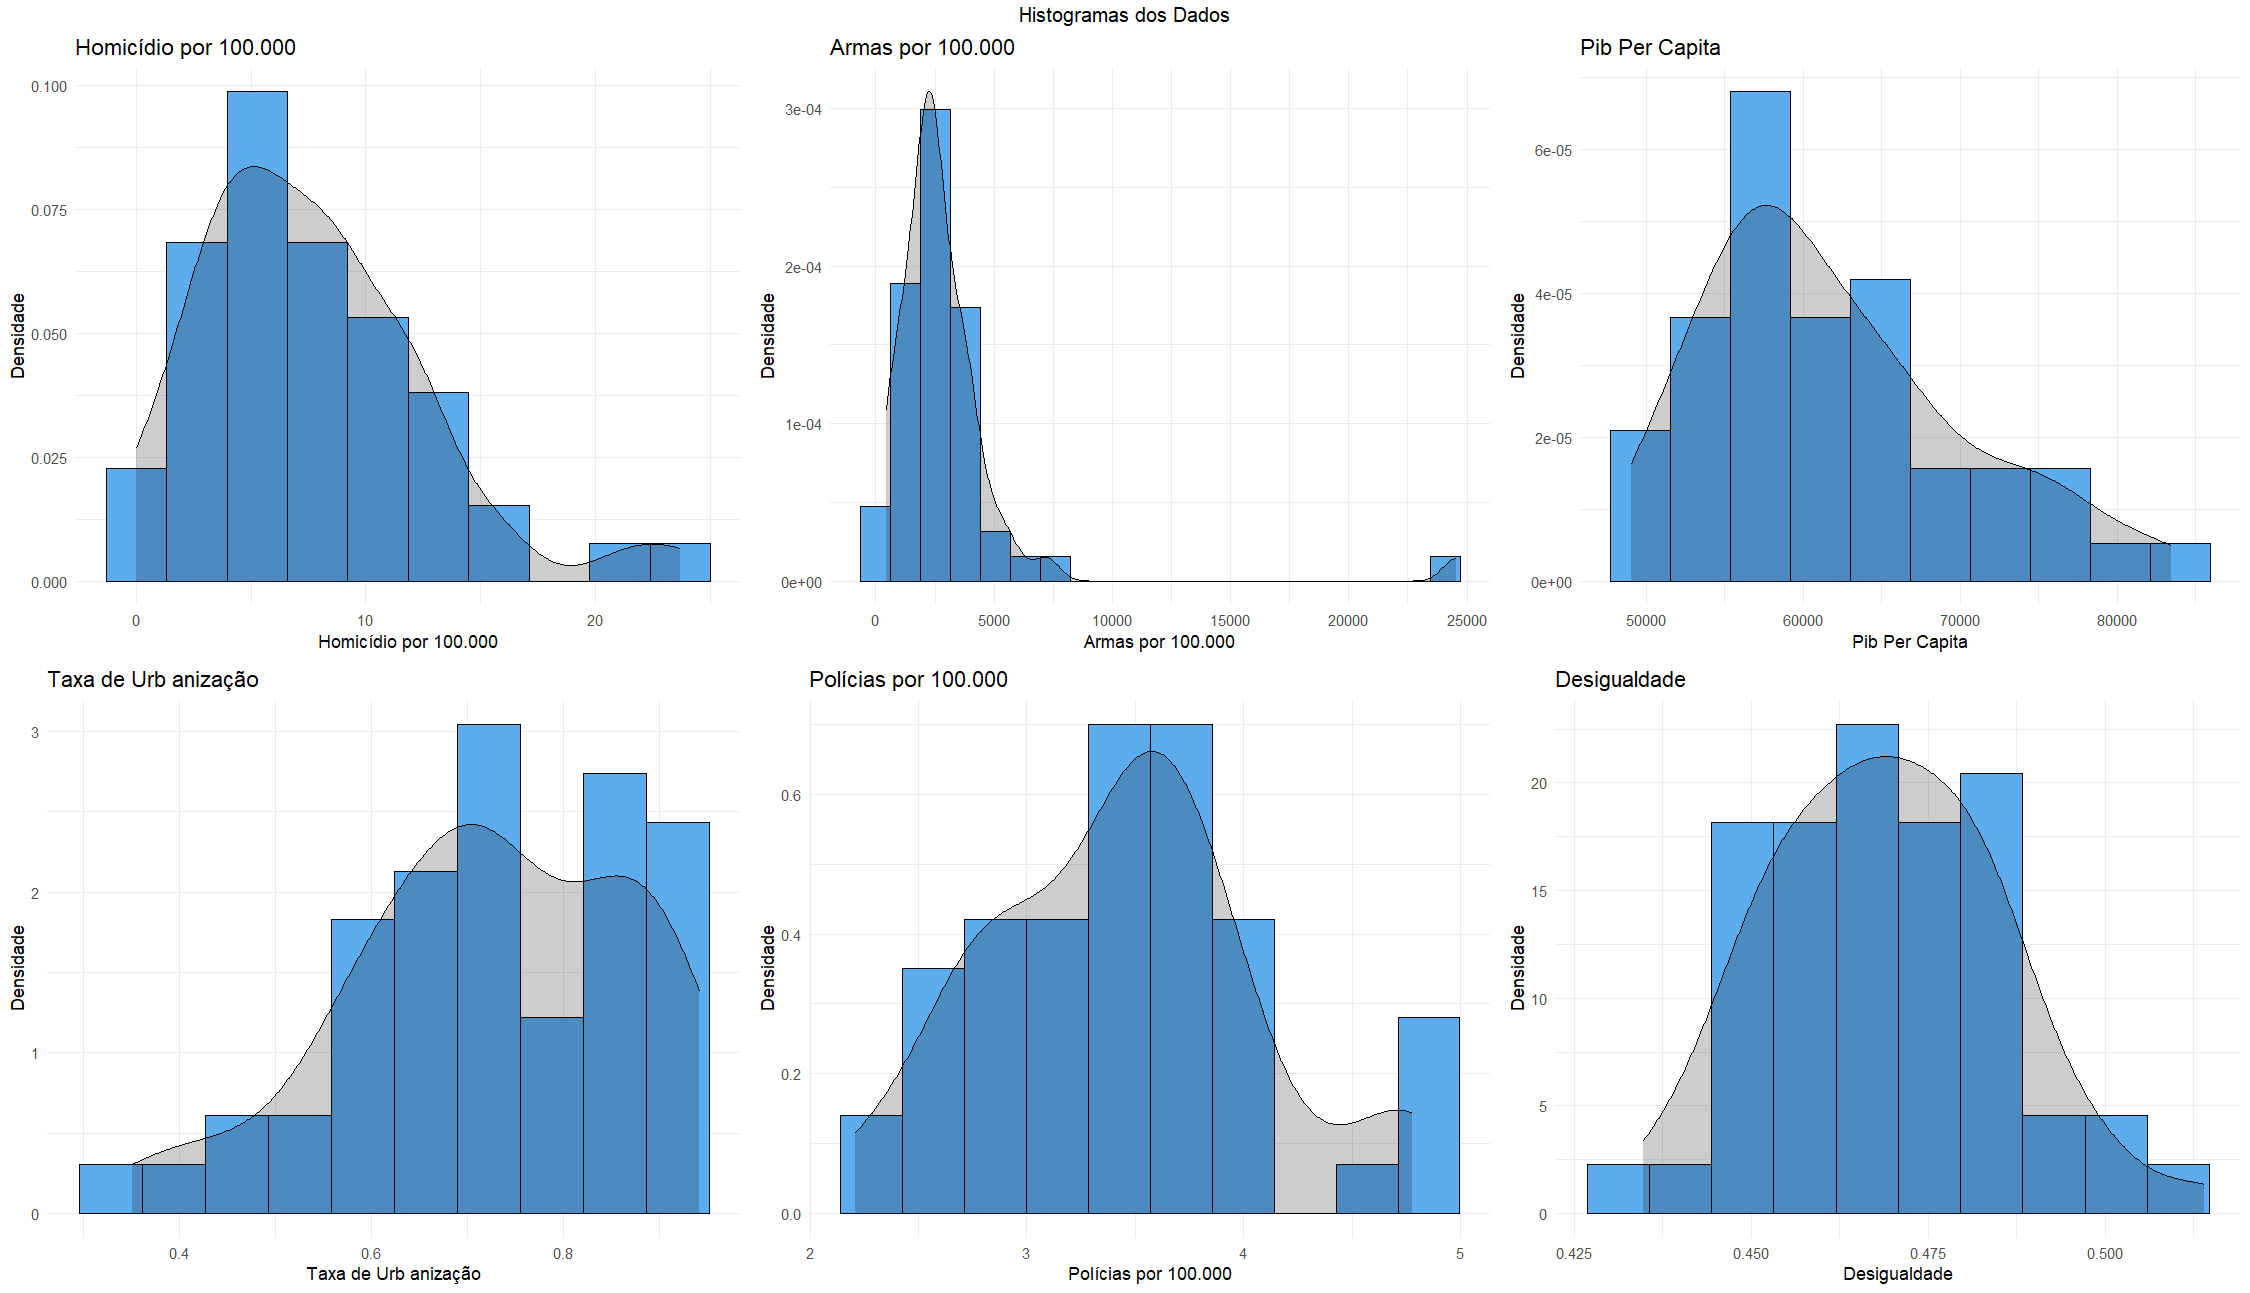
\includegraphics[width=1.0\textwidth]{Histograma do Dados.png}
    \label{fig:Histograma do Dados}
    
    \footnotesize{Fonte: Elaborado pelos autores.}
    \end{figure}

\begin{figure}[H]
    \centering
    \caption{Boxplot dos Dados}
    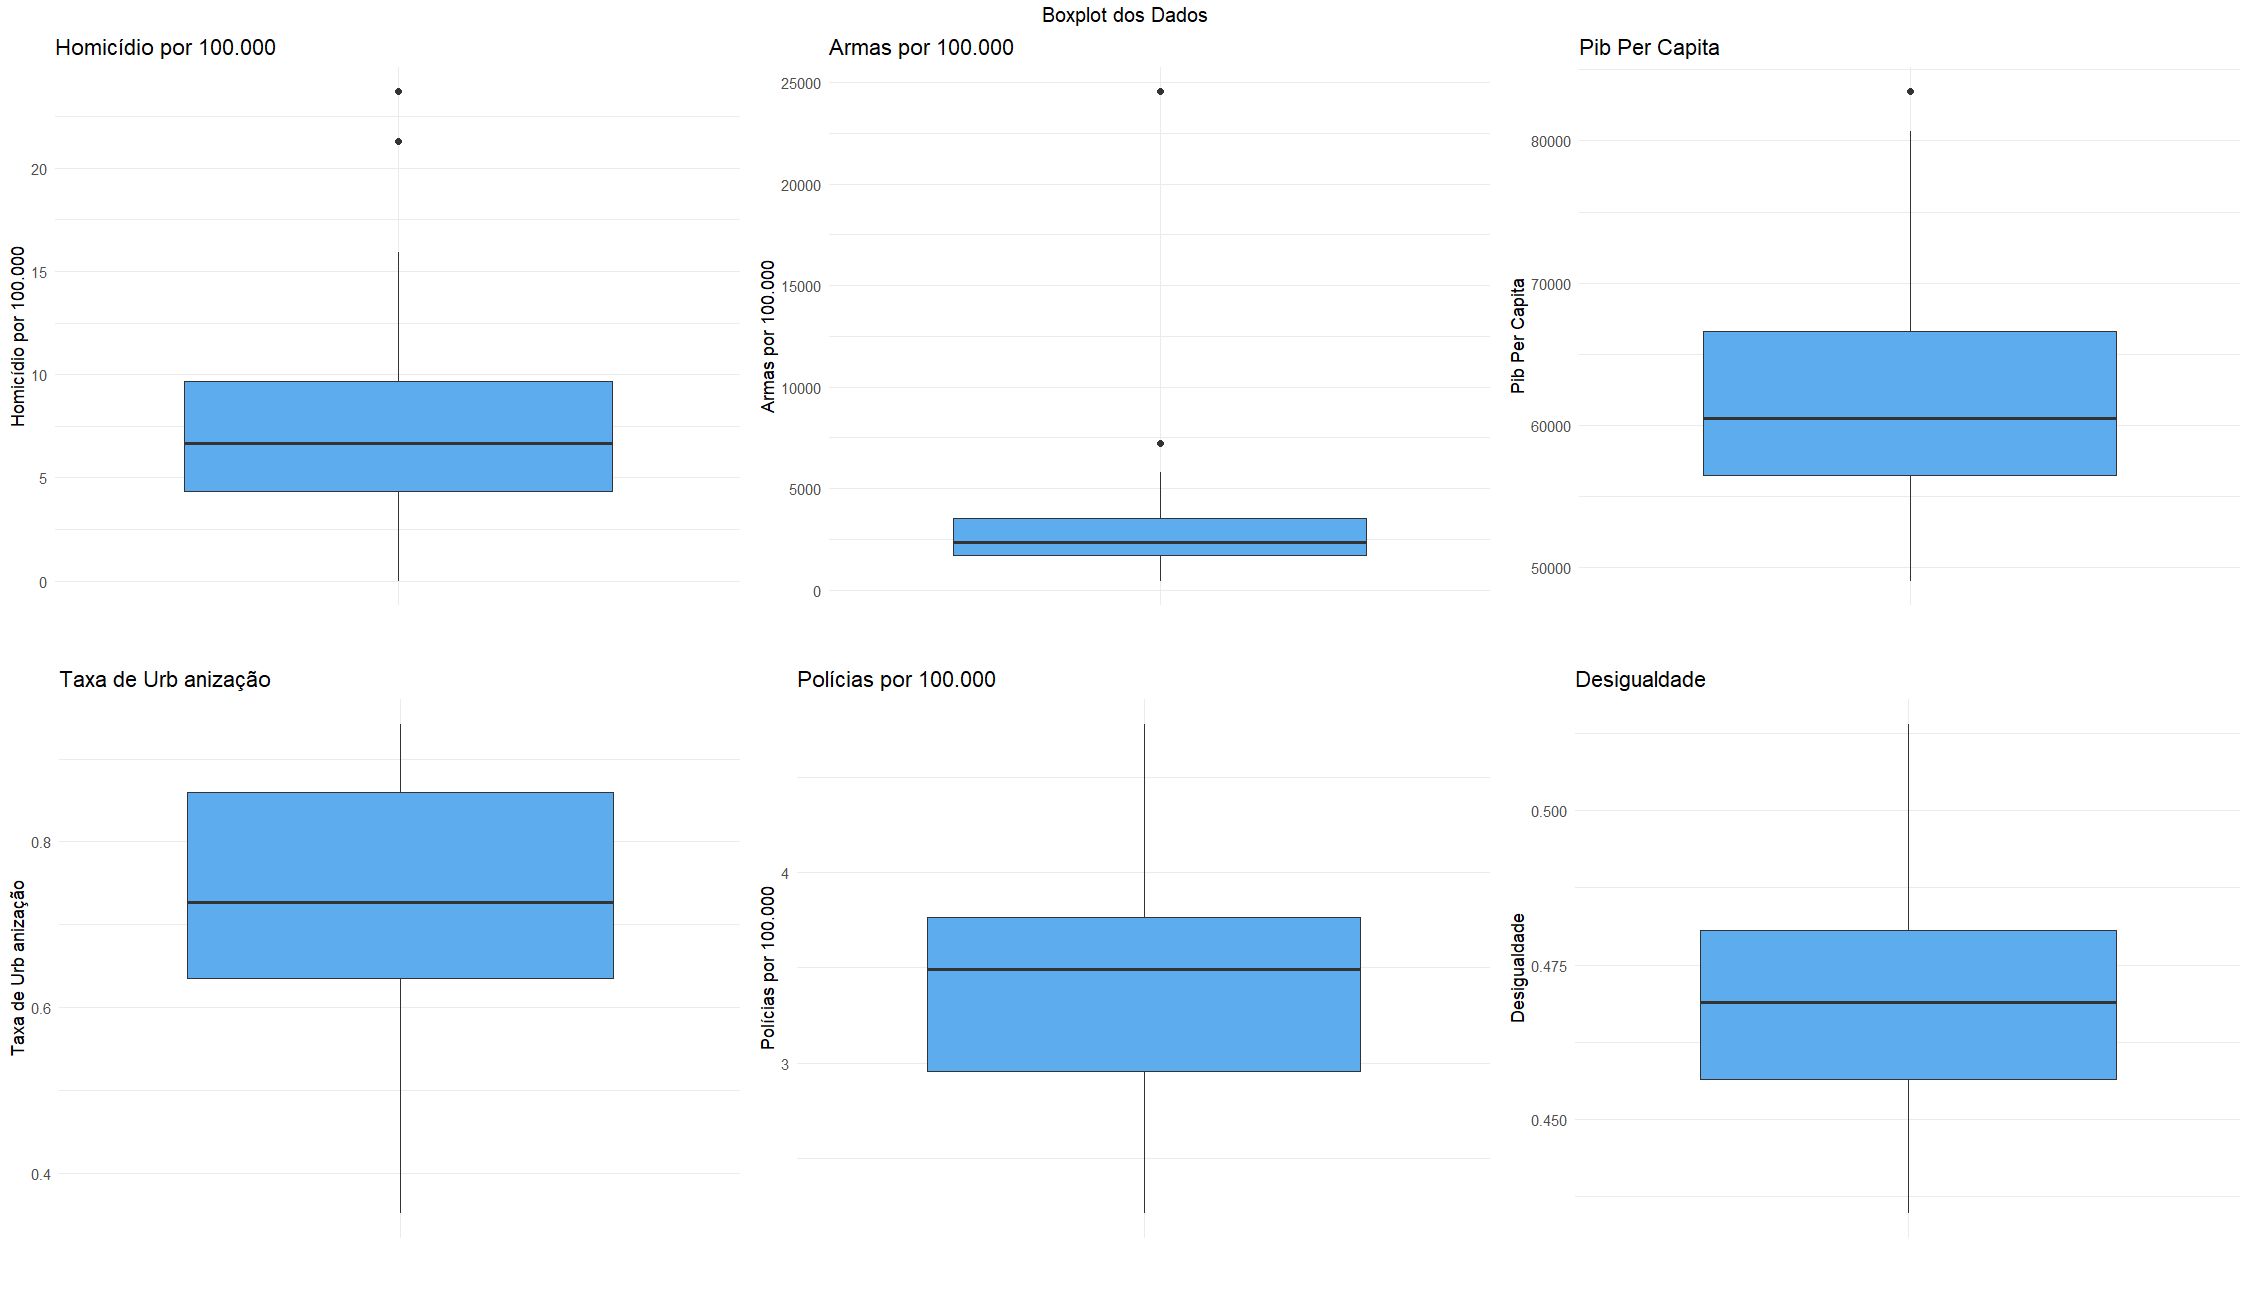
\includegraphics[width=1.0\textwidth]{Boxplot dos Dados.png}
    \label{fig:Boxplot dos Dados}
    
    \footnotesize{Fonte: Elaborado pelos autores.}
\end{figure}

\begin{figure}[H]
    \centering
    \caption{Comparação dos Boxplot das Armas com e sem Outliers}
    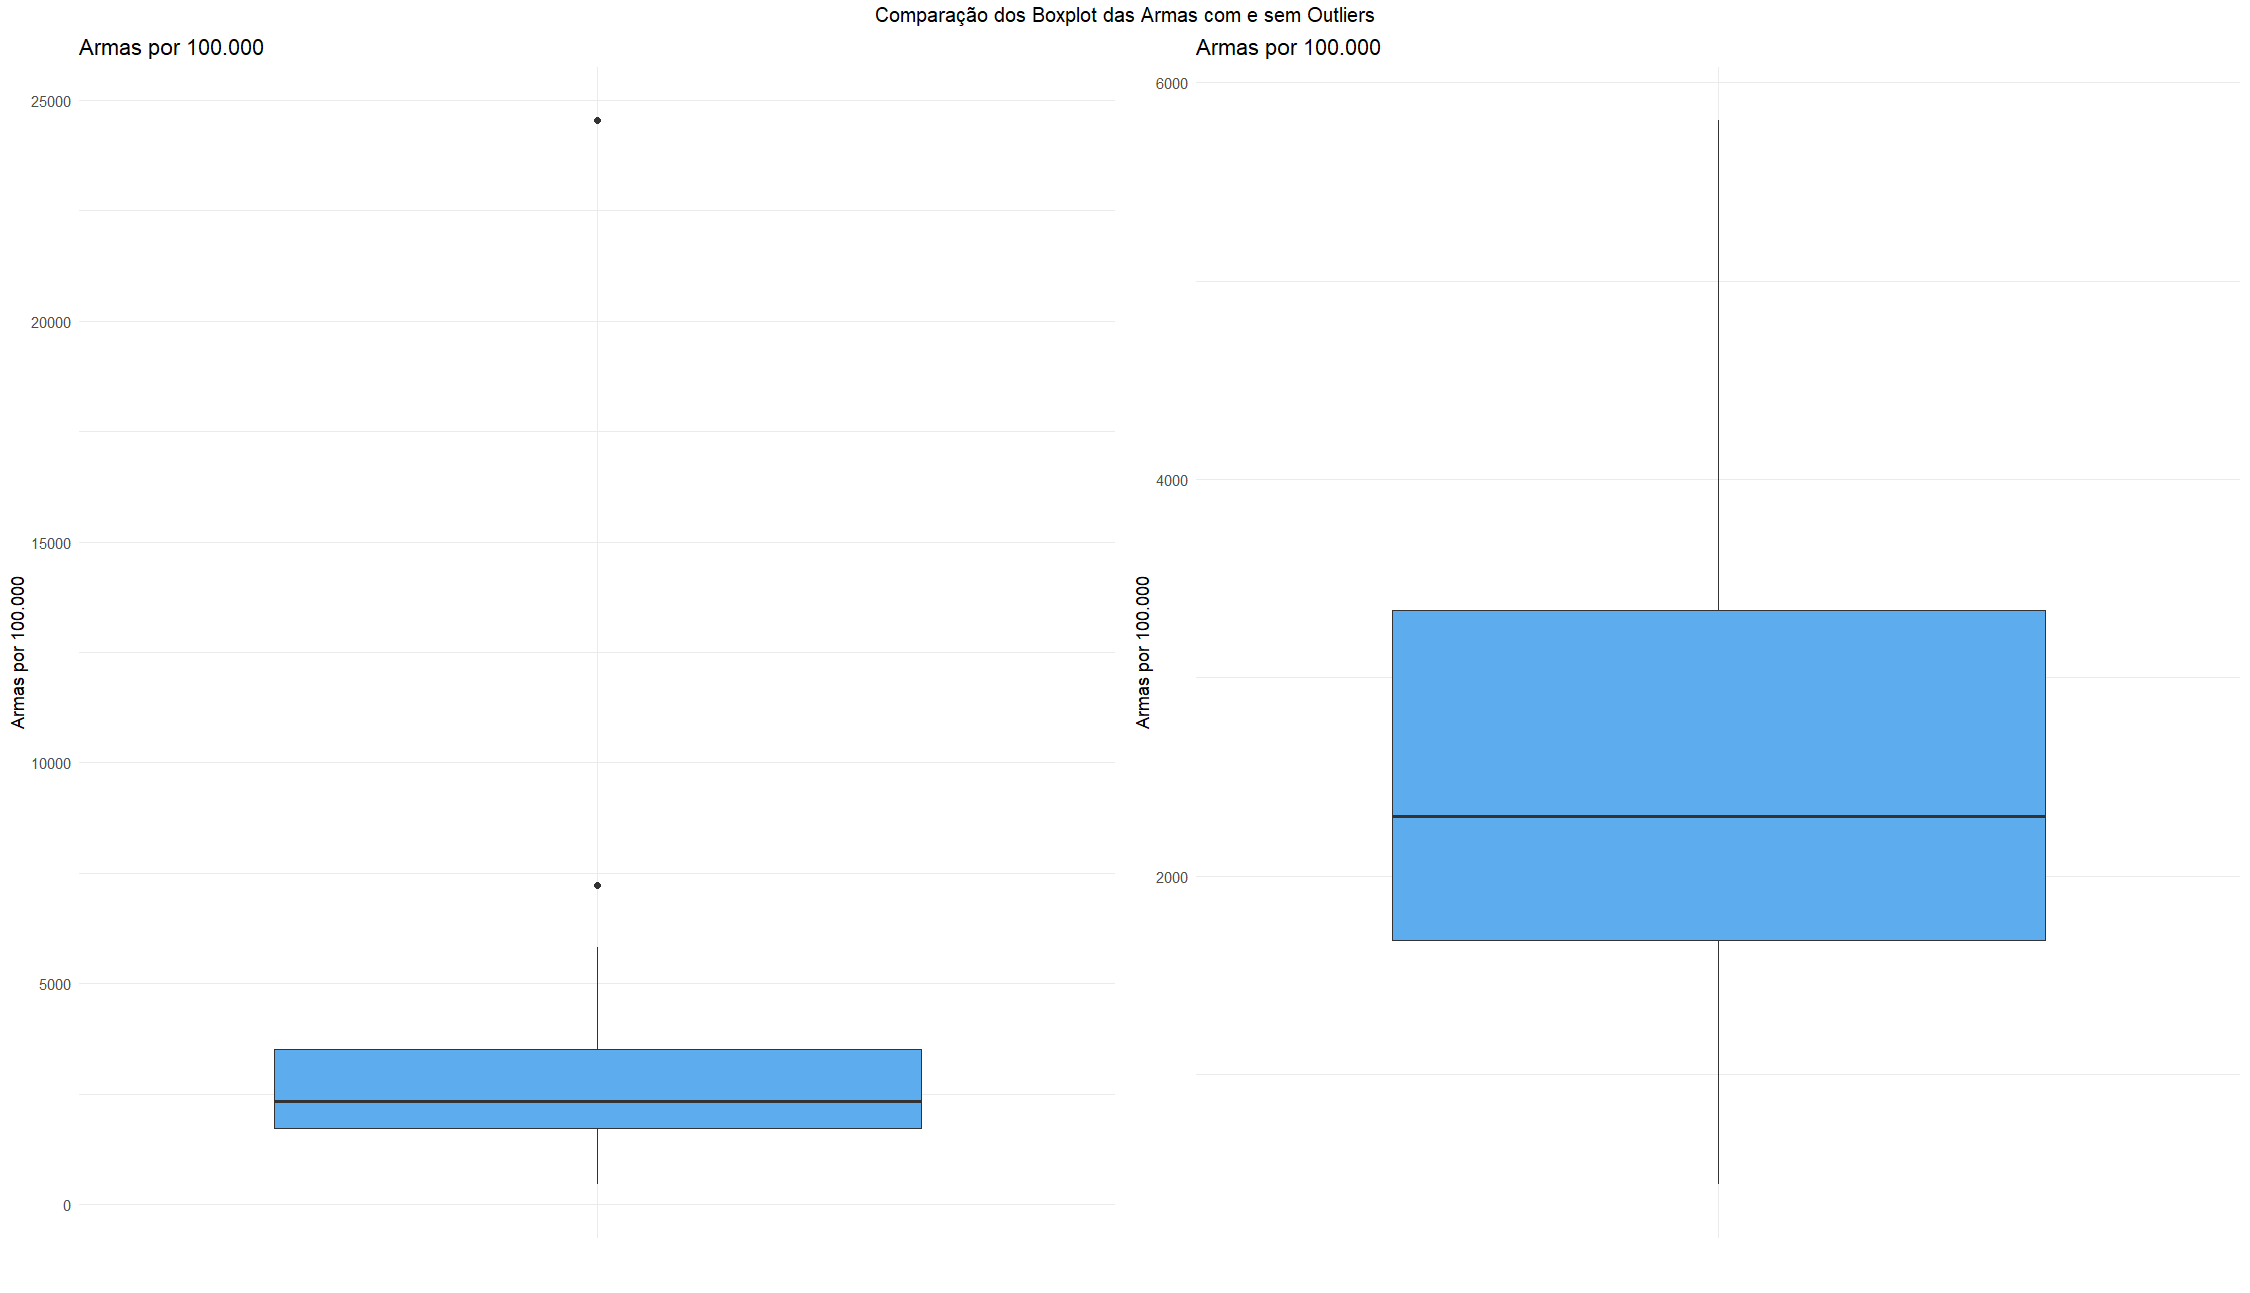
\includegraphics[width=1.0\textwidth]{Boxplot dos Dados sem Outlier.png}
    \label{fig:Boxplot dos Dados sem Outlier}
    
    \footnotesize{Fonte: Elaborado pelos autores.}
\end{figure}


\begin{figure}[H]
    \centering
    \caption{Matriz de Dispersão, Distribuição e Correlação}
    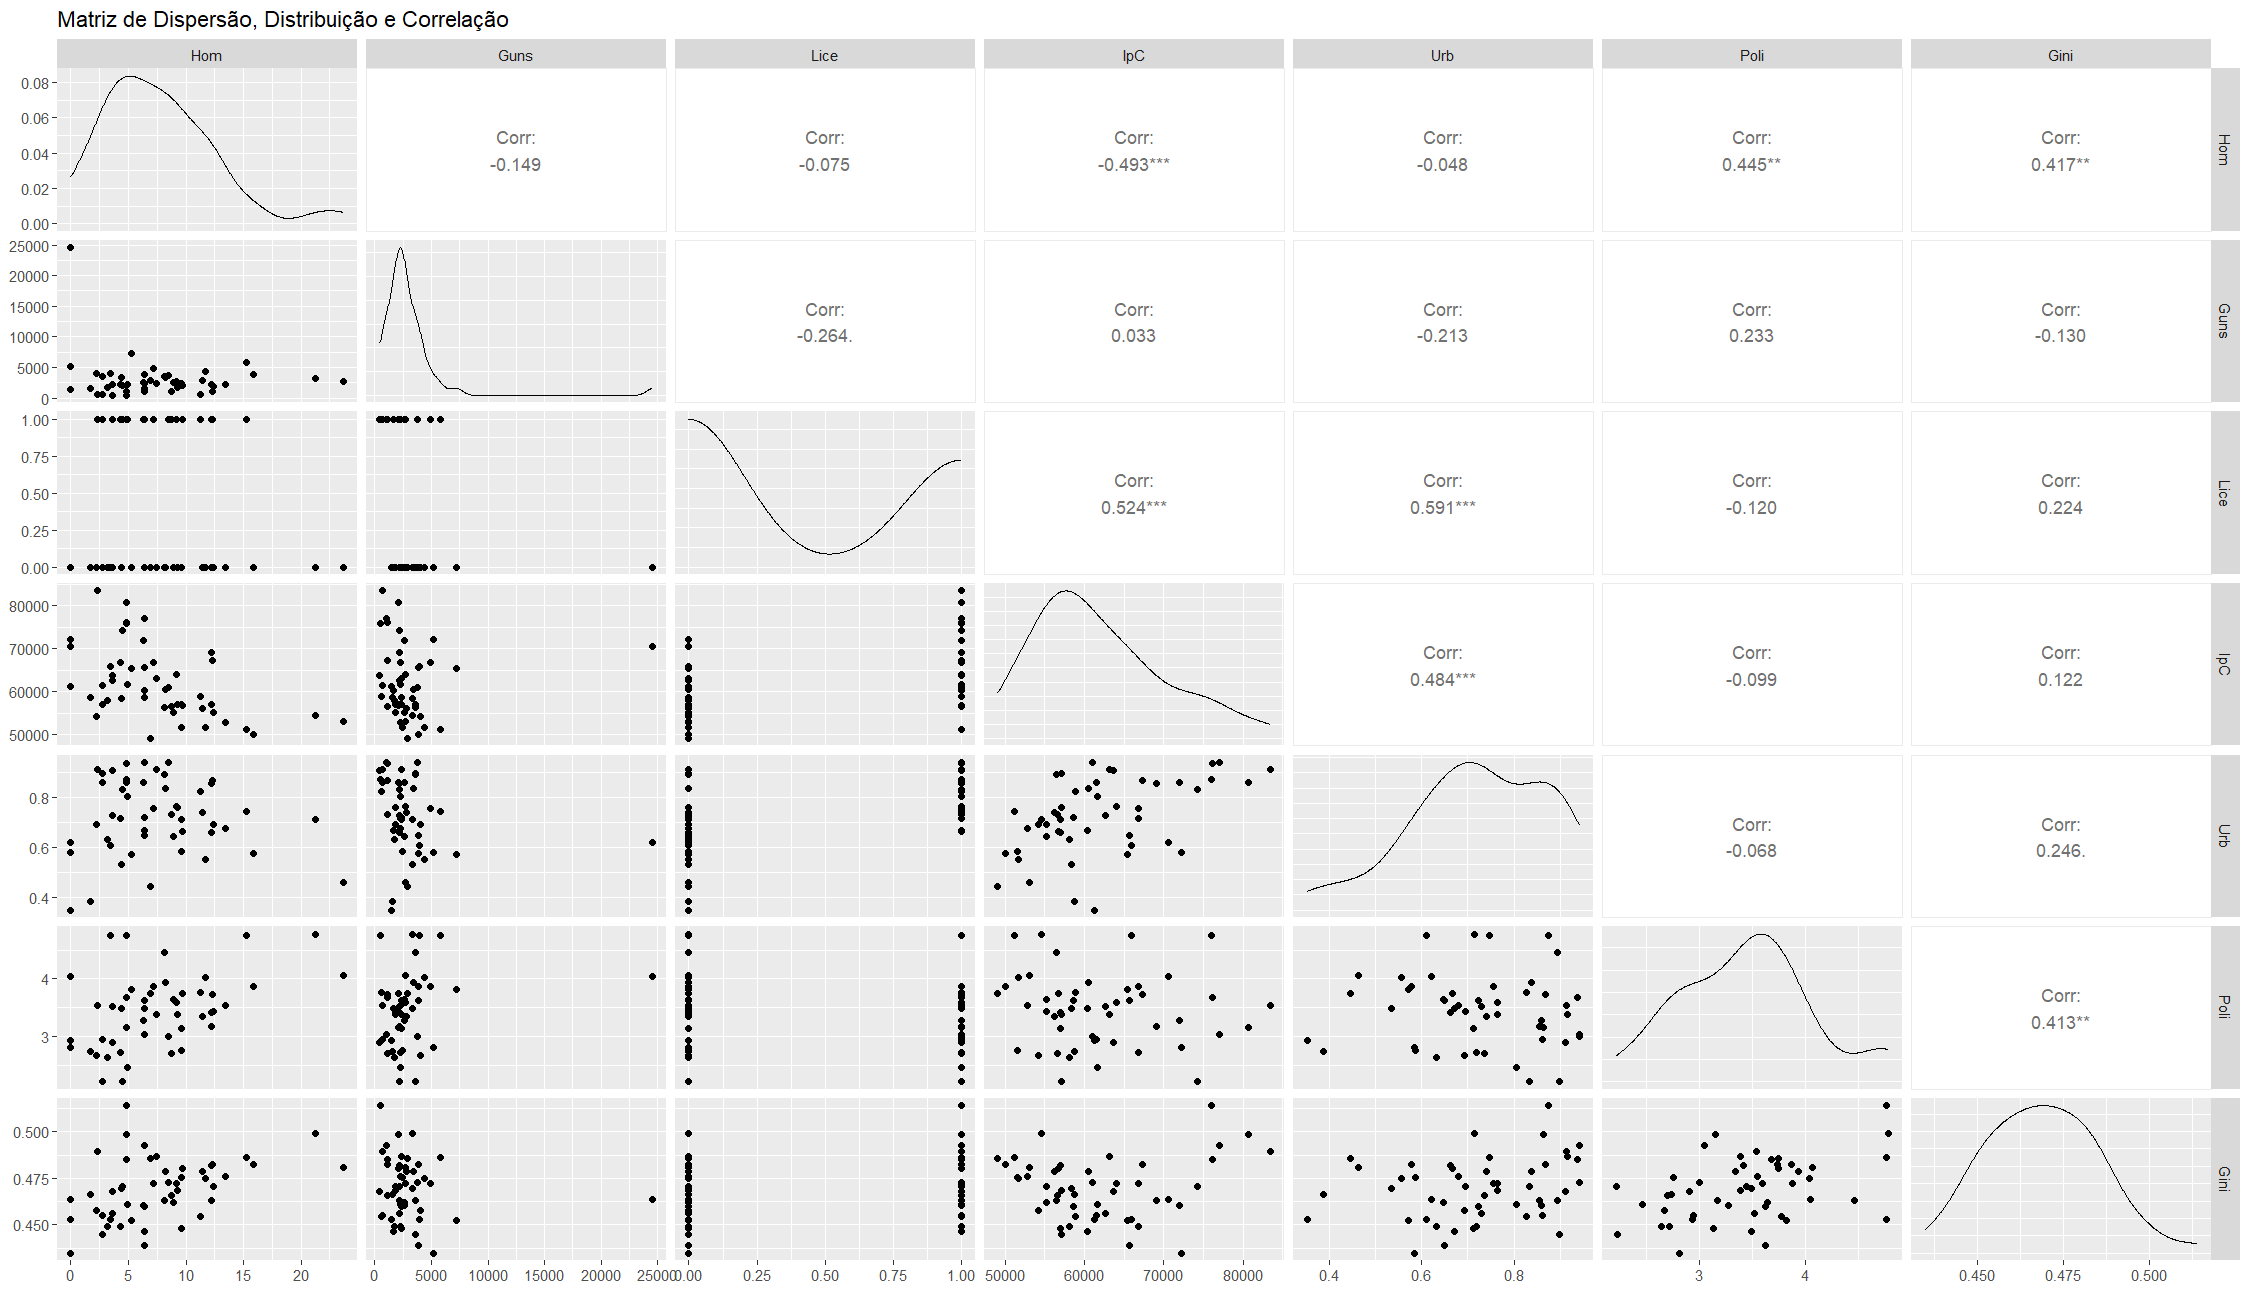
\includegraphics[width=1.0\textwidth]{Matriz de Dispersão, Distribuição e Correlação.png}
    \label{fig:Matriz de Dispersão, Distribuição e Correlação}
    
    \footnotesize{Fonte: Elaborado pelos autores.}
\end{figure}


\section{\textbf{Base de Dados sem Licença (Lice == 0)}}
\begin{table}[H]
\centering
\caption{Tabela Descritiva dos Dados sem Licença (Lice == 0)}
\label{tab:indicadores_sem_licença}
\small
\begin{tabularx}{\textwidth}{l*{6}{R}}
\hline
Indicador & Média & Mediana & Máximo & Mínimo & Variância & Desvio Padrão \\ \hline
Homicídio por 100.000 & 7.91 & 7.40 & 23.70 & 0.00 & 34.59 & 5.88 \\
Armas por 100.000 & 3782.64 & 2819.09 & 24547.23 & 1460.81 & 17441975.90 & 4176.36 \\
PIB Per Capita & 58230.52 & 57026.00 & 72214.00 & 49071.00 & 33122364.26 & 5755.20 \\
Taxa de Urbanização & 0.65 & 0.65 & 0.92 & 0.35 & 0.02 & 0.14 \\
Polícias por 100.000 & 3.51 & 3.52 & 4.78 & 2.22 & 0.39 & 0.62 \\
Desigualdade & 0.47 & 0.47 & 0.50 & 0.43 & 0.00 & 0.02 \\ \hline
\end{tabularx}
\footnotesize{Fonte: Elaborado pelos autores.}
\end{table}

\begin{table}[H]
\centering
\caption{Matriz de Correlação dos Dados sem Licença (Lice == 0)}
\label{tab:correlation_matrix_sem_licença}
\begin{tabular}{lrrrrrrr}
\hline
      & Hom   & Guns  & Lice  & IpC   & Urb   & Poli  & Gini  \\ \hline
Hom   & 1     & -0.27 &       & -0.61 & 0.07  & 0.46  & 0.69  \\
Guns  & -0.27 & 1     &       & 0.48  & -0.03 & 0.23  &-0.10  \\
Lice  &       &       & 1     &       &       &       &       \\
IpC   & -0.61 & 0.48  &       & 1     & 0.07  & 0.01  & -0.58 \\
Urb   & 0.07  & -0.03 &       & 0.07  & 1     & 0.05  & 0.03  \\
Poli  & 0.46  & 0.23  &       & 0.01  & 0.05  & 1     & 0.41  \\
Gini  & 0.69  & -0.10 &       & -0.58 & 0.03  & 0.41  & 1     \\ \hline
\end{tabular}
\end{table}

\begin{figure}[H]
    \centering
    \caption{Boxplot dos Dados que não têm Licença}
    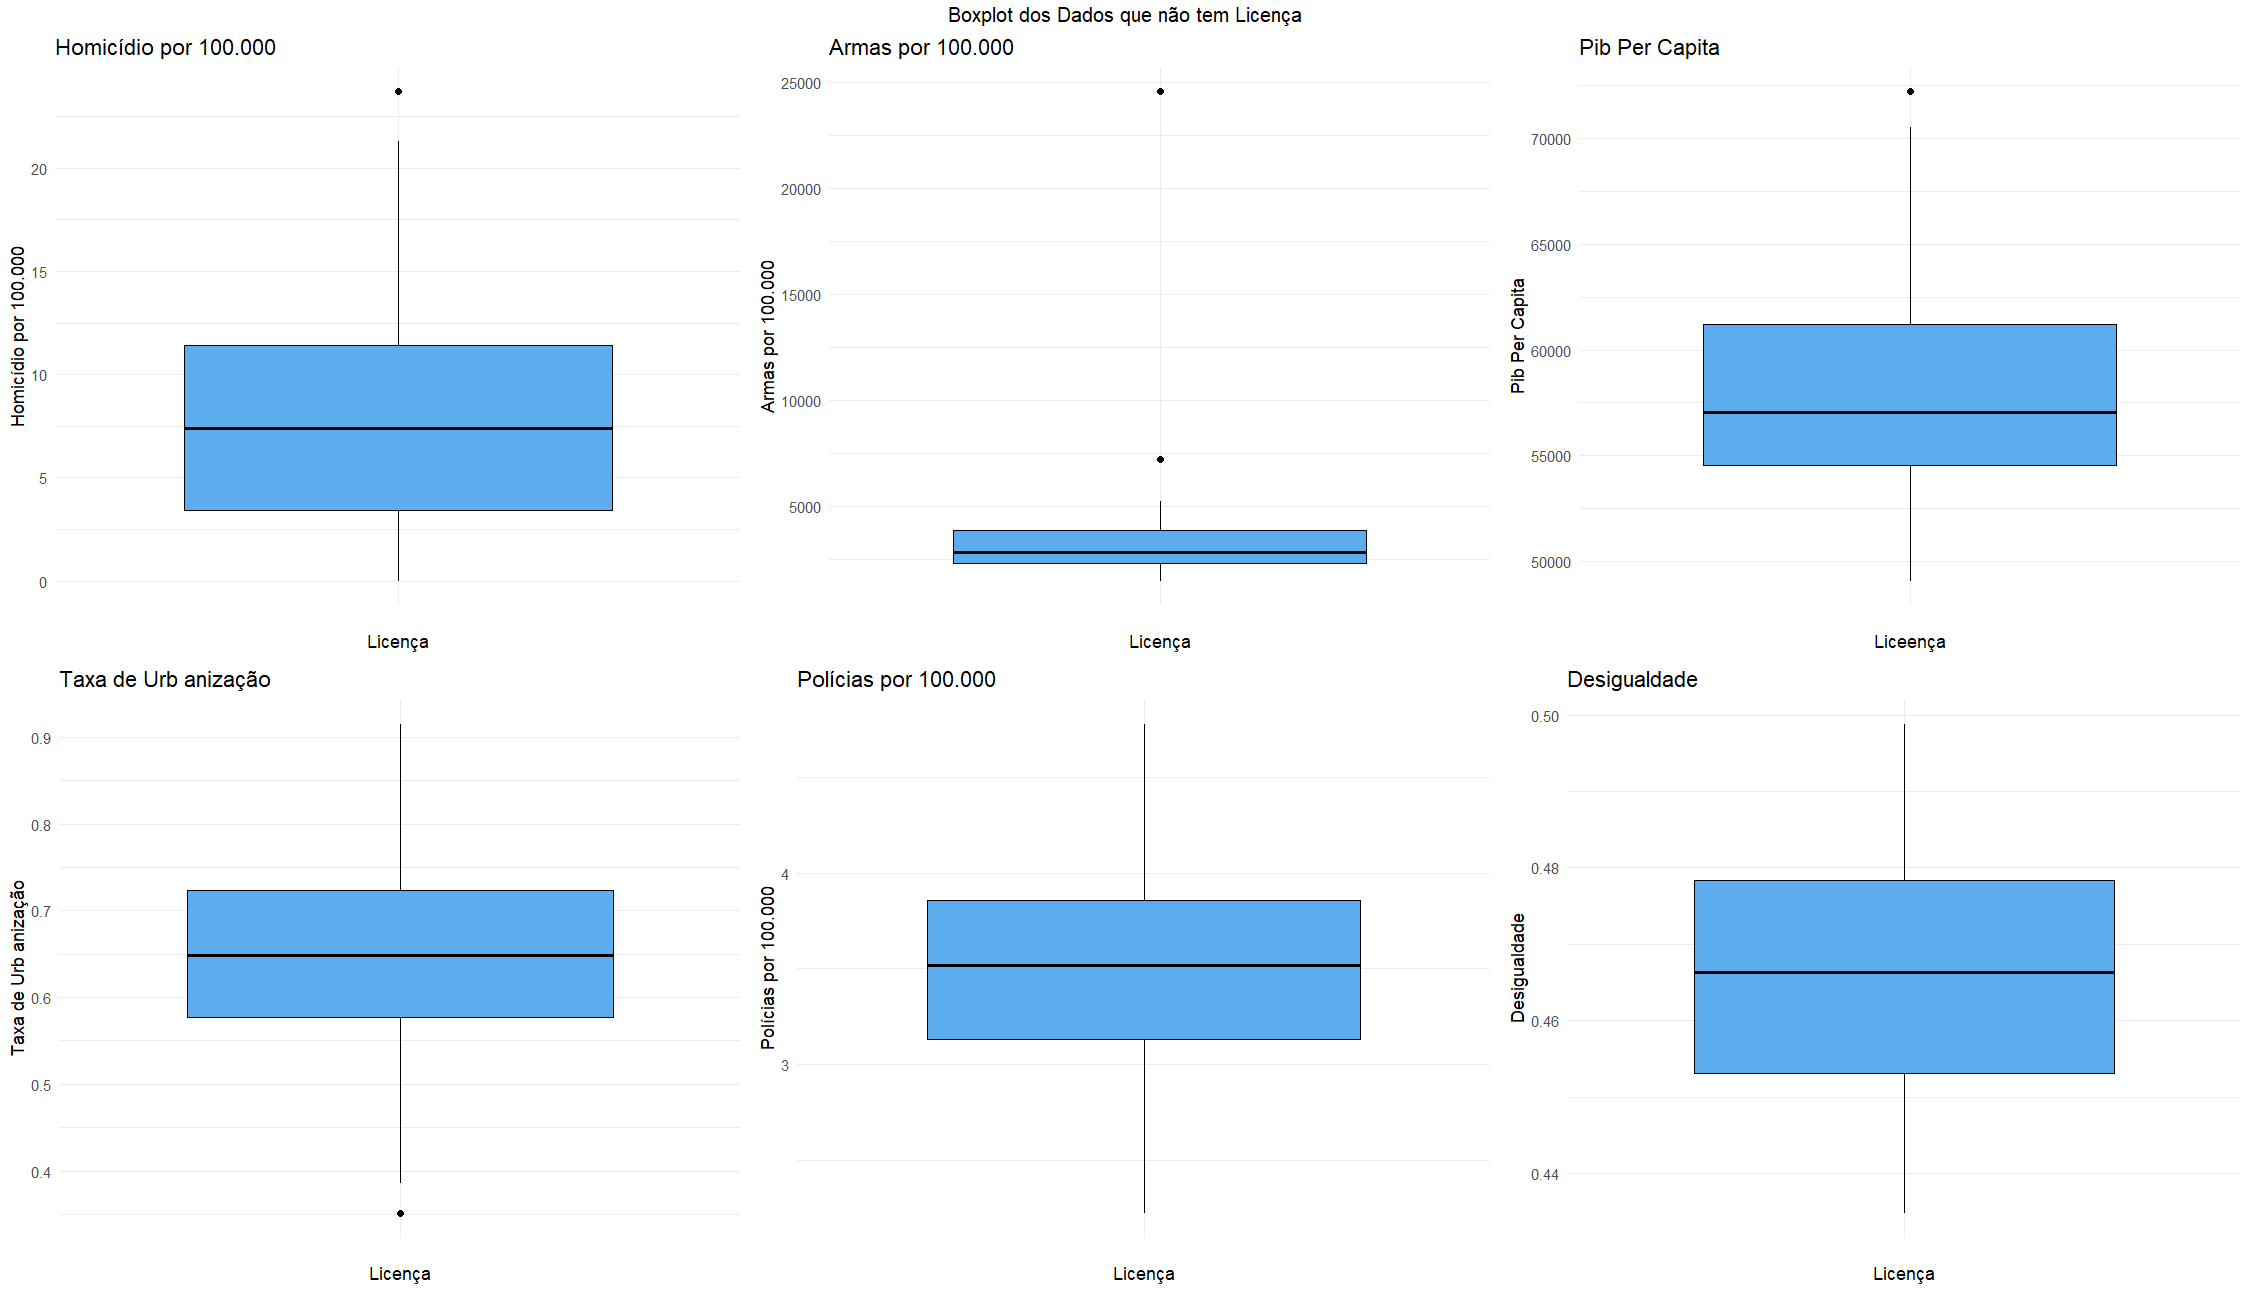
\includegraphics[width=1.0\textwidth]{Boxplot dos Dados que não tem Licença.png}
    \label{fig:Boxplot dos Dados que não tem Licença}
    
    \footnotesize{Fonte: Elaborado pelos autores.}
\end{figure}

\begin{figure}[H]
    \centering
    \caption{Histograma dos Dados que não têm Licença}
    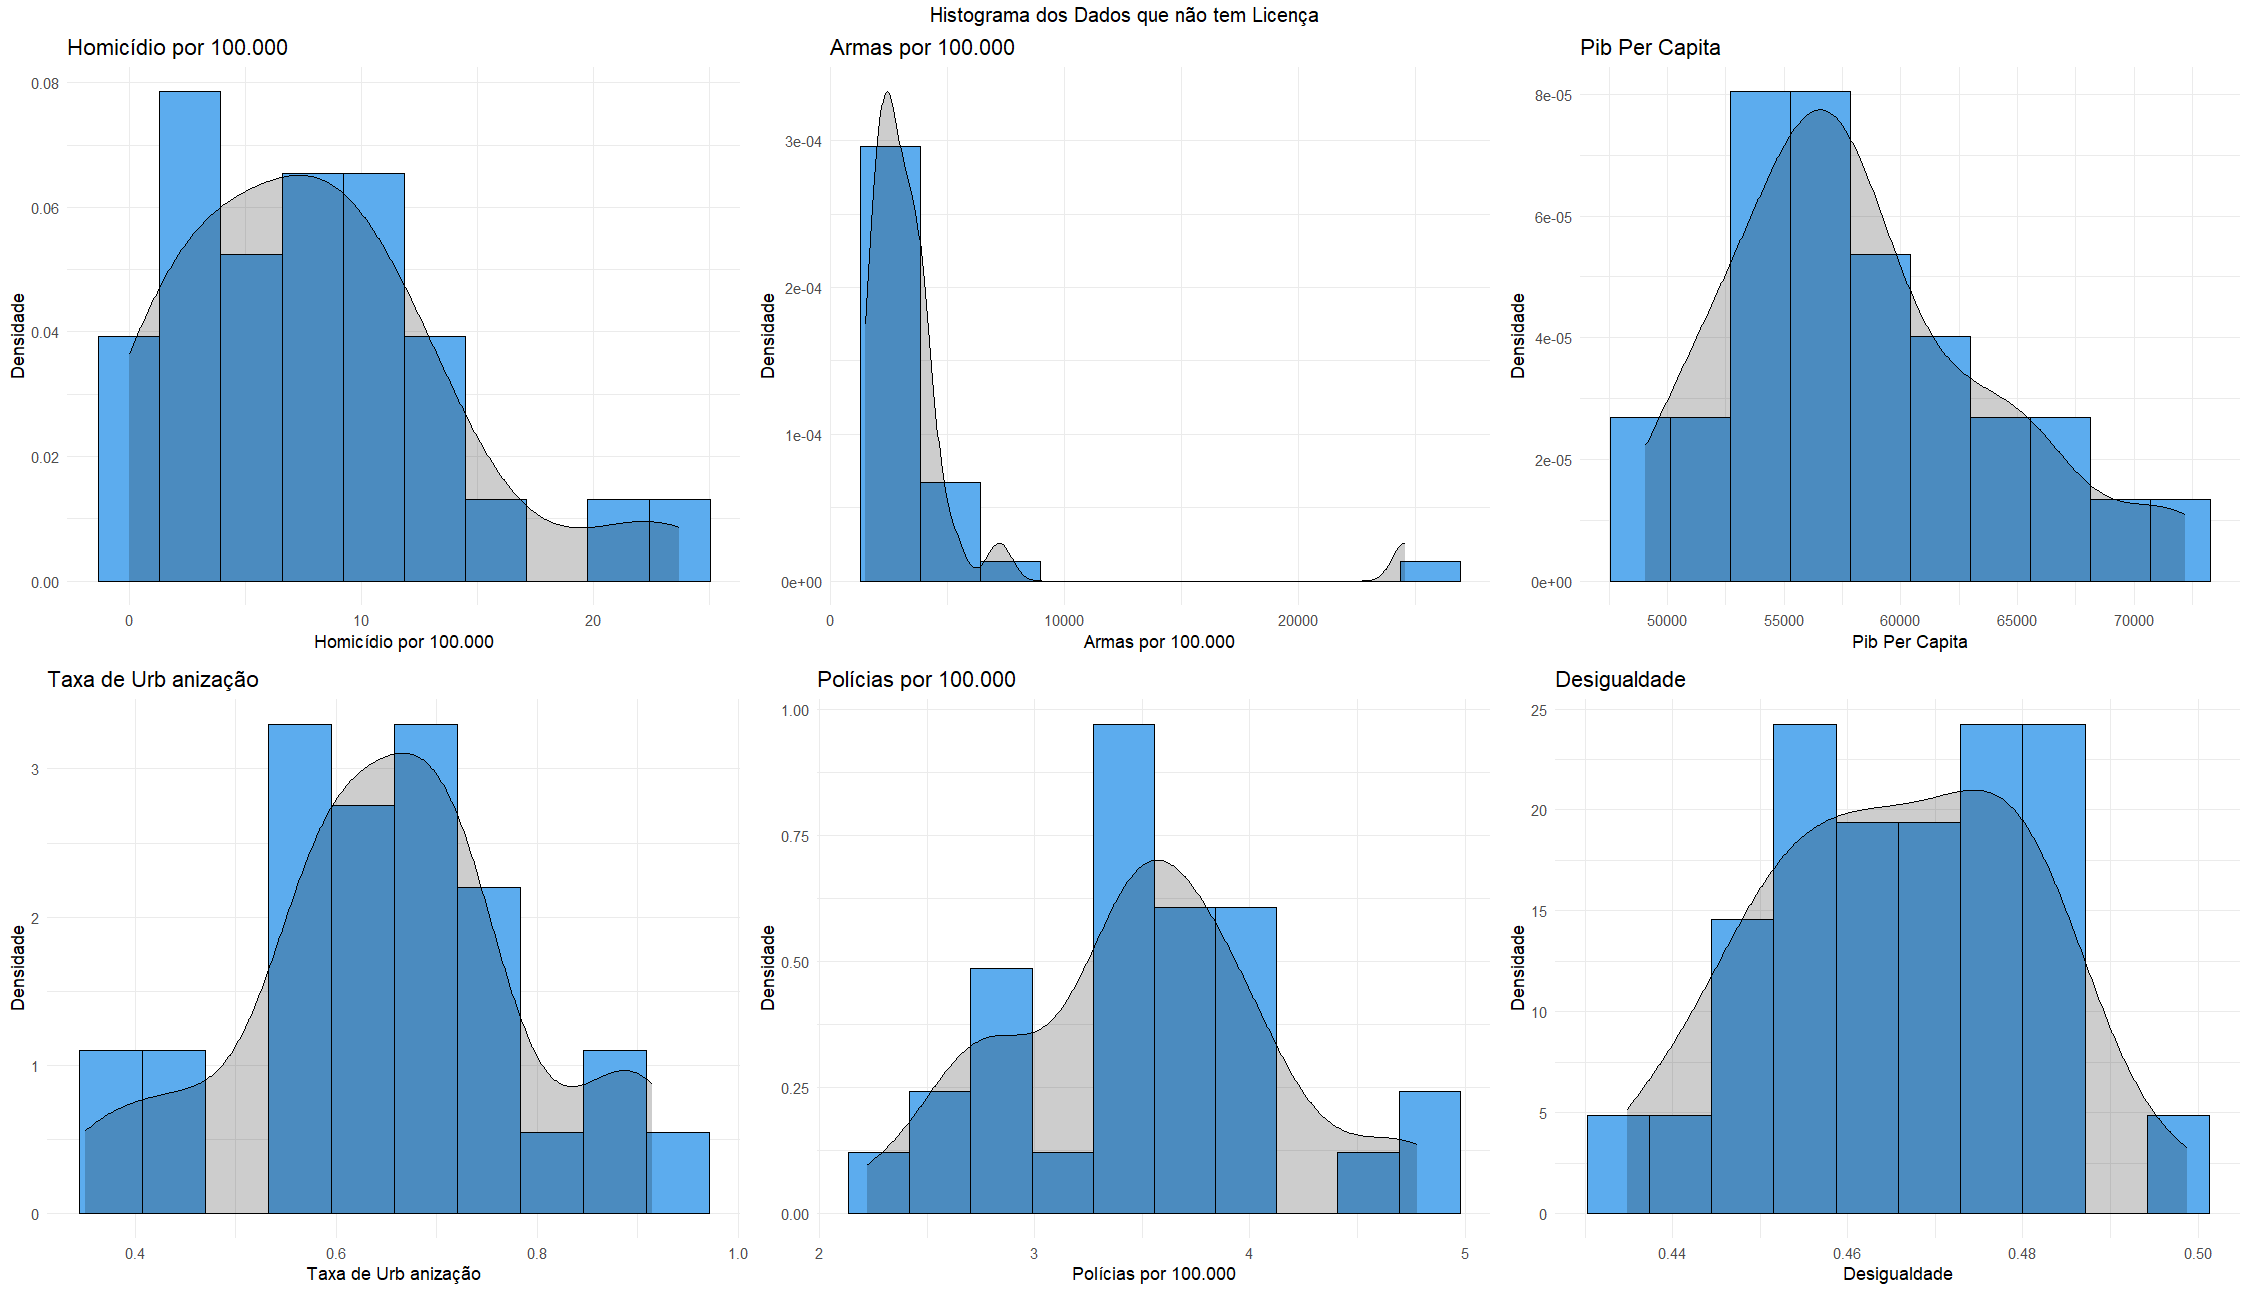
\includegraphics[width=1.0\textwidth]{Histograma dos Dados que não tem Licença.png}
    \label{fig:Histograma dos Dados que não tem Licença}
    
    \footnotesize{Fonte: Elaborado pelos autores.}
\end{figure}


\section{\textbf{Base de Dados com Licença (Lice == 1)}}
\begin{table}[H]
\centering
\caption{Tabela Descritiva dos Dados com Licença (Lice == 1)}
\label{tab:indicadores_com_licença}
\small
\begin{tabularx}{\textwidth}{l*{6}{R}}
\hline
Indicador & Média & Mediana & Máximo & Mínimo & Variância & Desvio Padrão \\ \hline
Homicídio por 100.000 & 7.15 & 6.40 & 15.30 & 2.30 & 12.26 & 3.50 \\
Armas por 100.000 & 1981.53 & 2066.43 & 5809.48 & 445.49 & 2045169.98 & 1430.09 \\
PIB Per Capita & 66897.67 & 66838.00 & 83461.00 & 51141.00 & 74544422.23 & 8633.91 \\
Taxa de Urbanização & 0.83 & 0.86 & 0.94 & 0.67 & 0.01 & 0.09 \\
Polícias por 100.000 & 3.36 & 3.27 & 4.76 & 2.21 & 0.43 & 0.65 \\
Desigualdade & 0.47 & 0.47 & 0.51 & 0.45 & 0.00 & 0.02 \\ \hline
\end{tabularx}
\footnotesize{Fonte: Elaborado pelos autores.}
\end{table}

\begin{table}[H]
\centering
\caption{Matriz de Correlação dos Dados com Licença (Lice == 1)}
\label{tab:correlation_matrix_com_licença}
\begin{tabular}{lrrrrrrr}
\hline
      & Hom   & Guns  & Lice  & IpC   & Urb   & Poli  & Gini  \\ \hline
Hom   & 1     & 0.47  &       & -0.56 & -0.3  & 0.44  & -0.01 \\
Guns  & 0.47  & 1     &       & -0.36 & -0.34 & 0.23  & -0.04 \\
Lice  &       &       & 1     &       &       &       &       \\
IpC   & -0.56 & -0.36 &       & 1     & 0.6   & -0.09 & 0.51  \\
Urb   & -0.3  & -0.34 &       & 0.6   & 1     & -0.11 & 0.41  \\
Poli  & 0.44  & 0.23  &       & -0.09 & -0.11 & 1     & 0.5   \\
Gini  & -0.01 & -0.04 &       & 0.51  & 0.41  & 0.5   & 1     \\ \hline
\end{tabular}
\end{table}

\begin{figure}[H]
    \centering
    \caption{Boxplot dos Dados que têm Licença}
    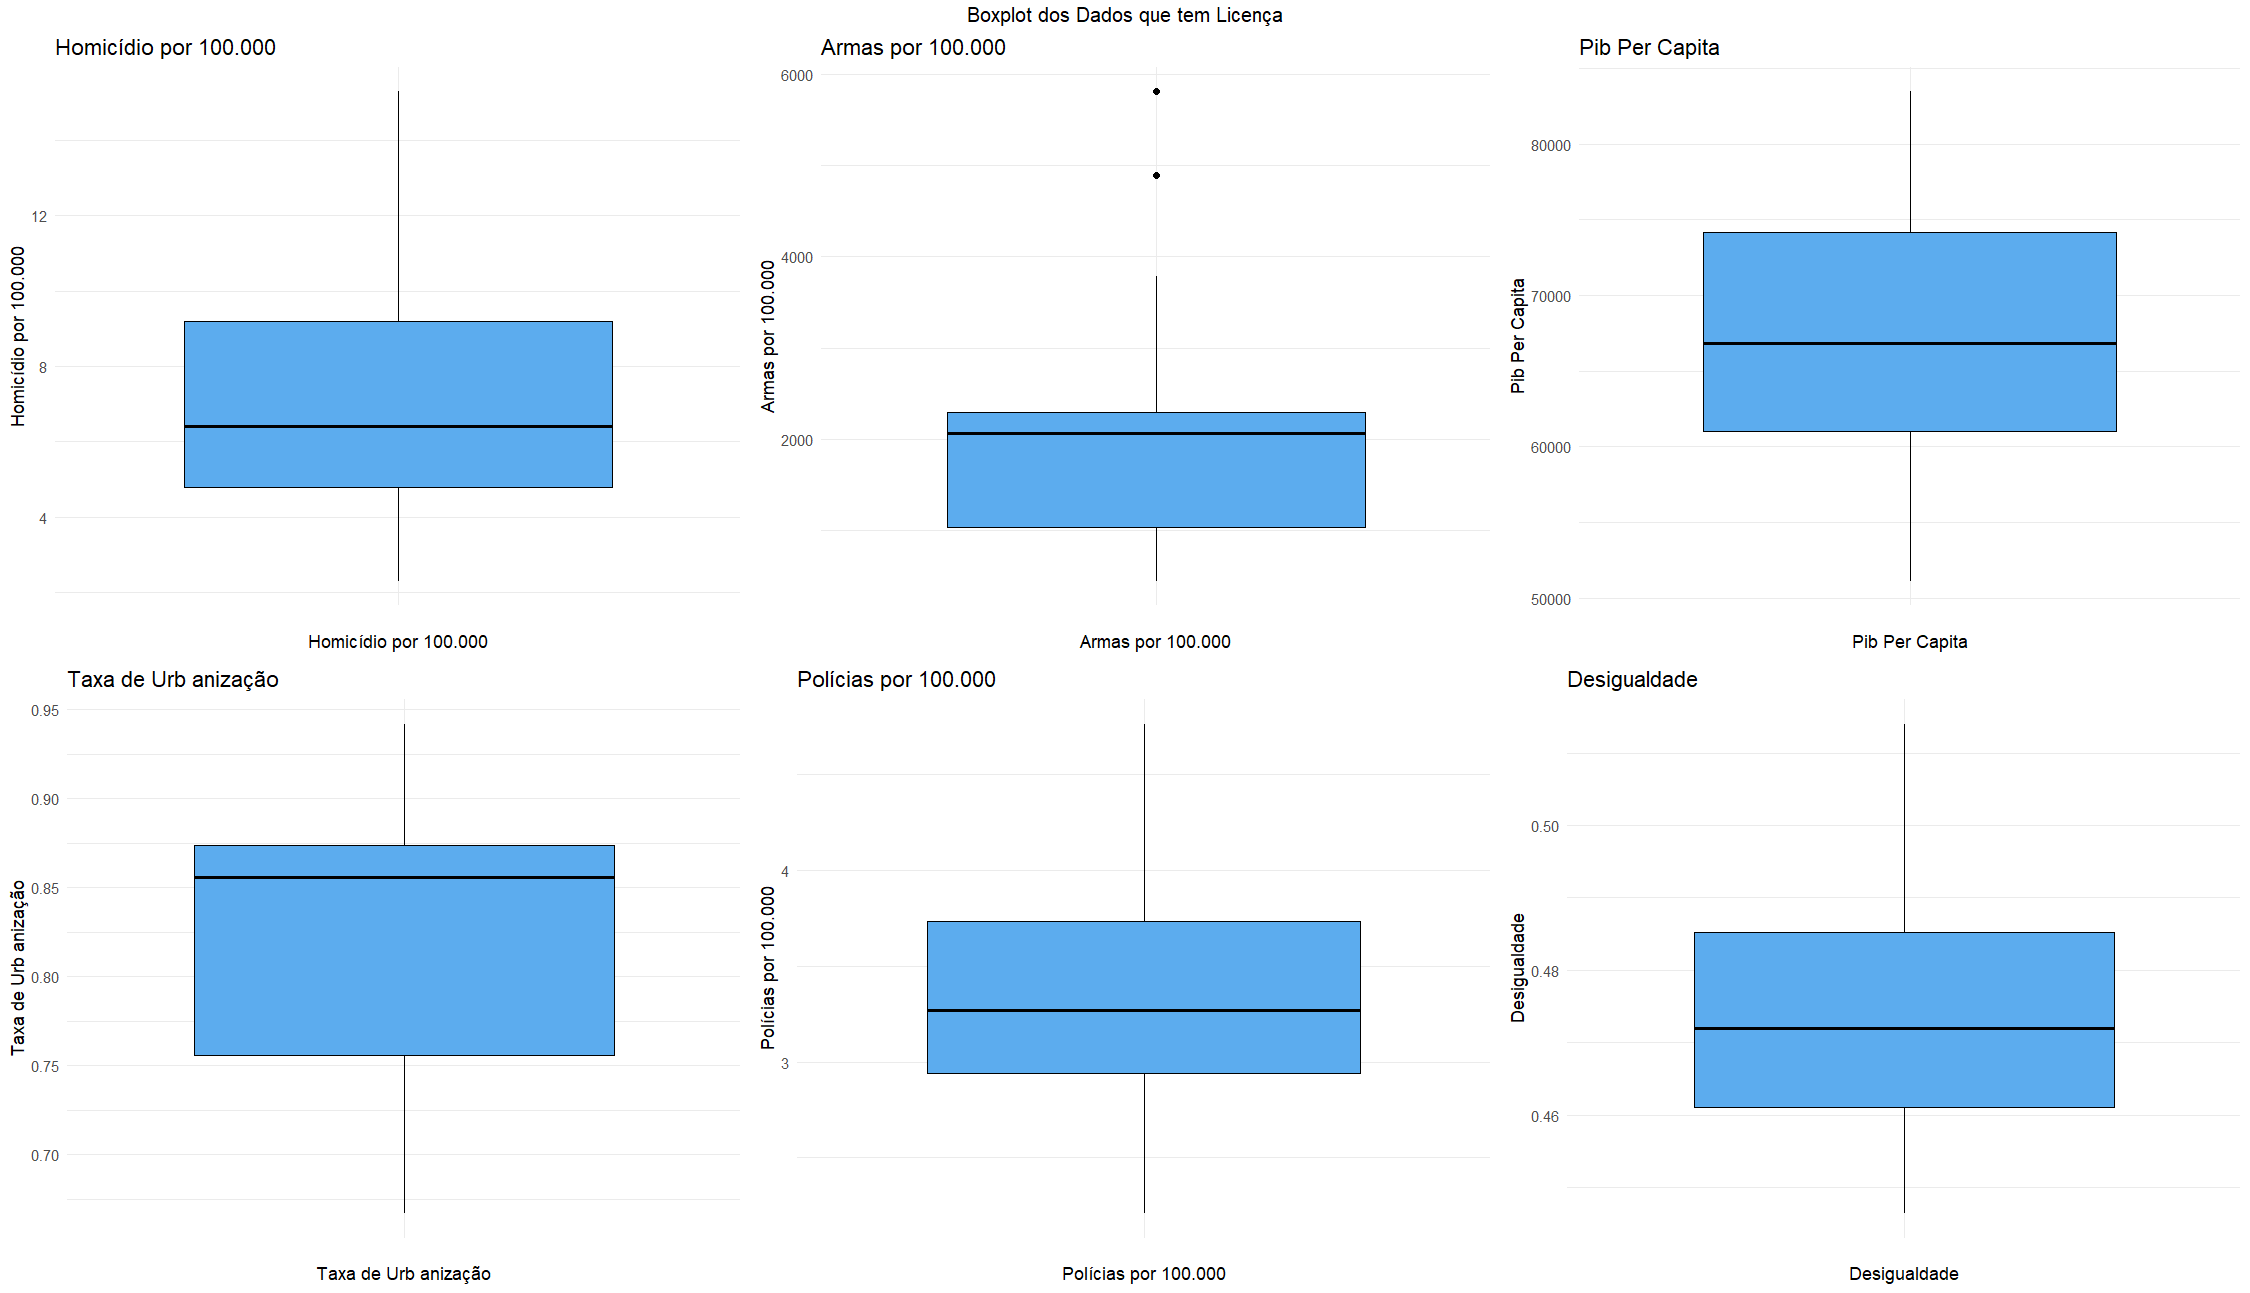
\includegraphics[width=1.0\textwidth]{Boxplot dos Dados que tem Licença.png}
    \label{fig:Boxplot dos Dados que tem Licença}
    
    \footnotesize{Fonte: Elaborado pelos autores.}
\end{figure}

\begin{figure}[H]
    \centering
    \caption{Histograma dos Dados que têm Licença}
    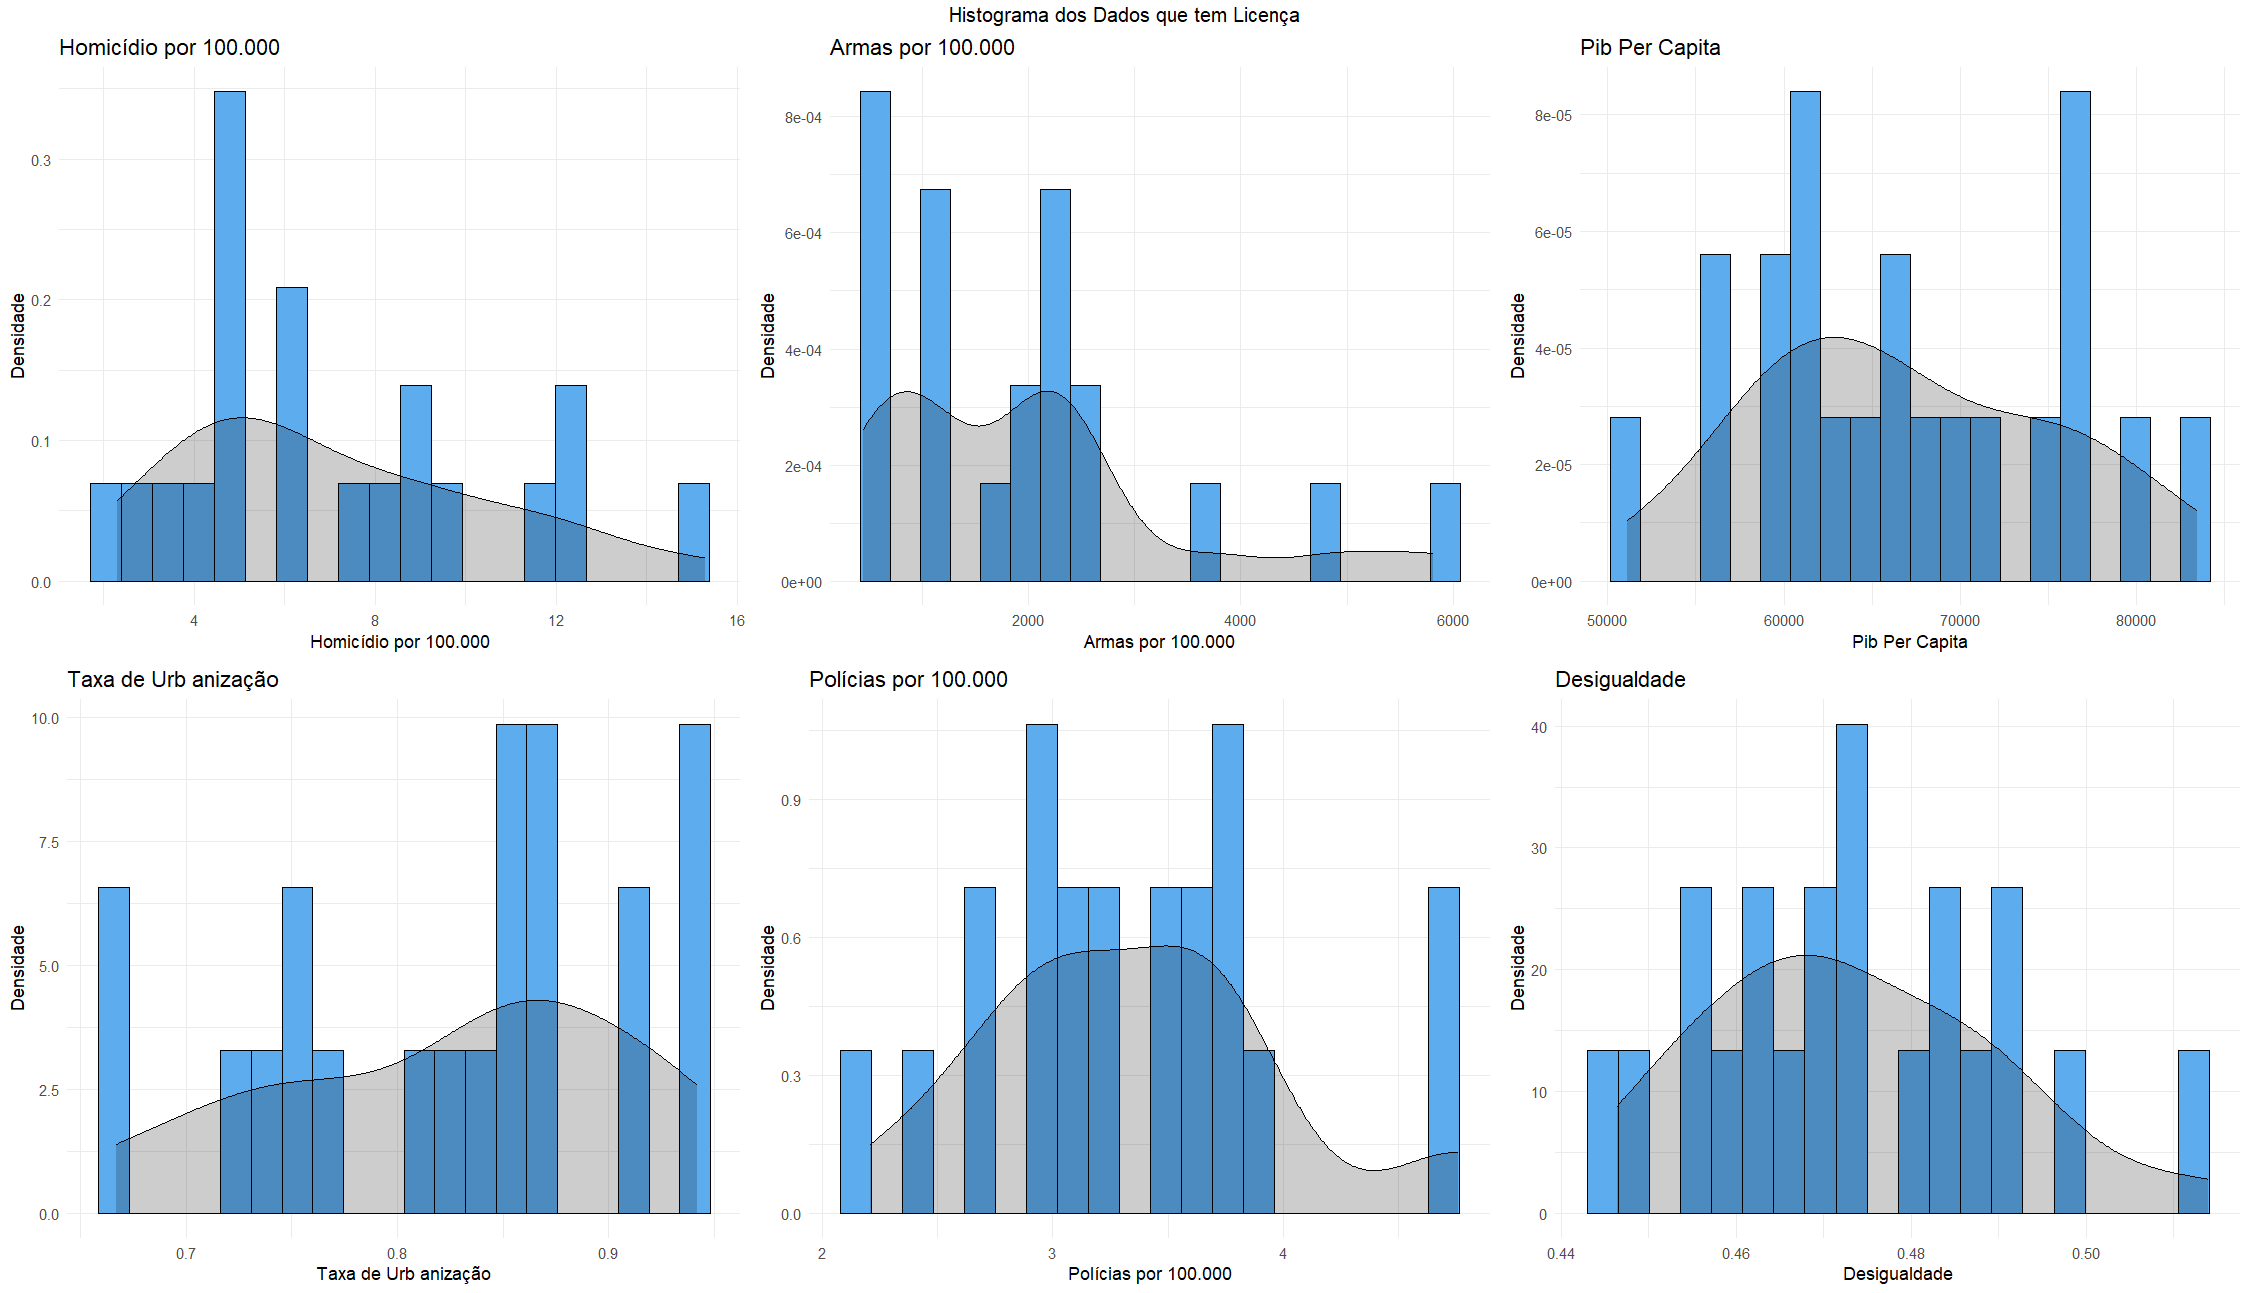
\includegraphics[width=1.0\textwidth]{Histograma dos Dados que tem Licença.png}
    \label{fig:Histograma dos Dados que tem Licença}
    
    \footnotesize{Fonte: Elaborado pelos autores.}
\end{figure}

\section{\textbf{Mapa dos Estados Unidos dada os Homicídios}}
\begin{figure}[H]
    \centering
    \caption{Mapa dos Estados Unidos dada a Homicídios}
    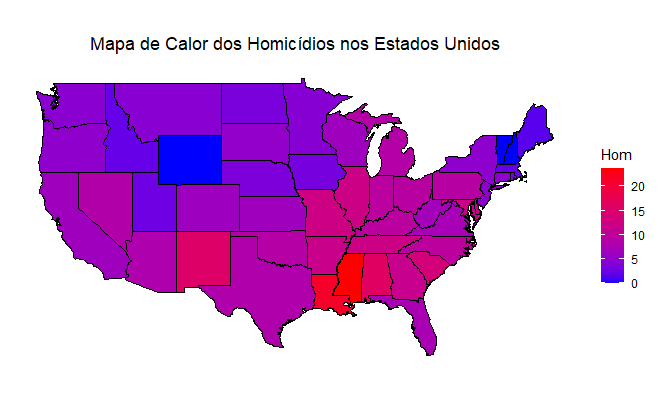
\includegraphics[width=1.0\textwidth]{image.png}
    \label{fig:Mapa dos Estados Unidos dada a Homicídios}
    
    \footnotesize{Fonte: Elaborado pelos autores.}
\end{figure}

\end{document}